\par L'itération 3 à ajoutée les expressions booléennes avec l'instruction si vaen. Et les commandes permettent d'enregistrer et charger un programme LIR dans l'interpréteur (commande charge et sauve).

\section{Diagrammes d'objets}
\begin{center}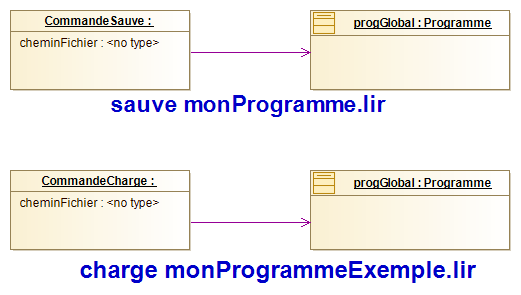
\includegraphics[scale=0.80]{./img/COO/COO_prototype_3/digrammesObjet/charge}\end{center}
\par Les commandes sauve et charge sont liées au programme pour pouvoir charger ou récupérer des lignes de codes. Ces commandes connaissent une chaînes de texte correspondant au chemin du fichier.
\par
\begin{center}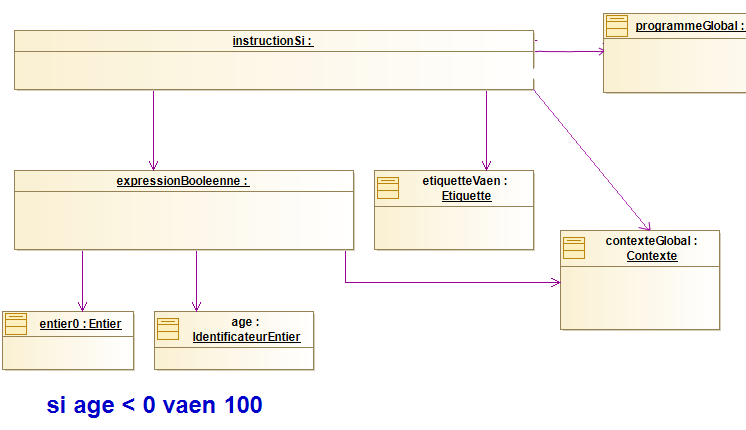
\includegraphics[scale=0.75]{./img/COO/COO_prototype_3/digrammesObjet/siVaen}\end{center}
\par L'instruction si a besoin pour fonctionner d'une ExpressionBooleenne et de connaitre le contexte pour chercher les valeurs des variables à comparer. Elle doit connaitre l'étiquette où aller si la condition est vraie et donc du programme pour appeler la méthode du programme vaen.

\section{Paquetage interpreteurlir.donnees(.litteraux)}
\begin{center}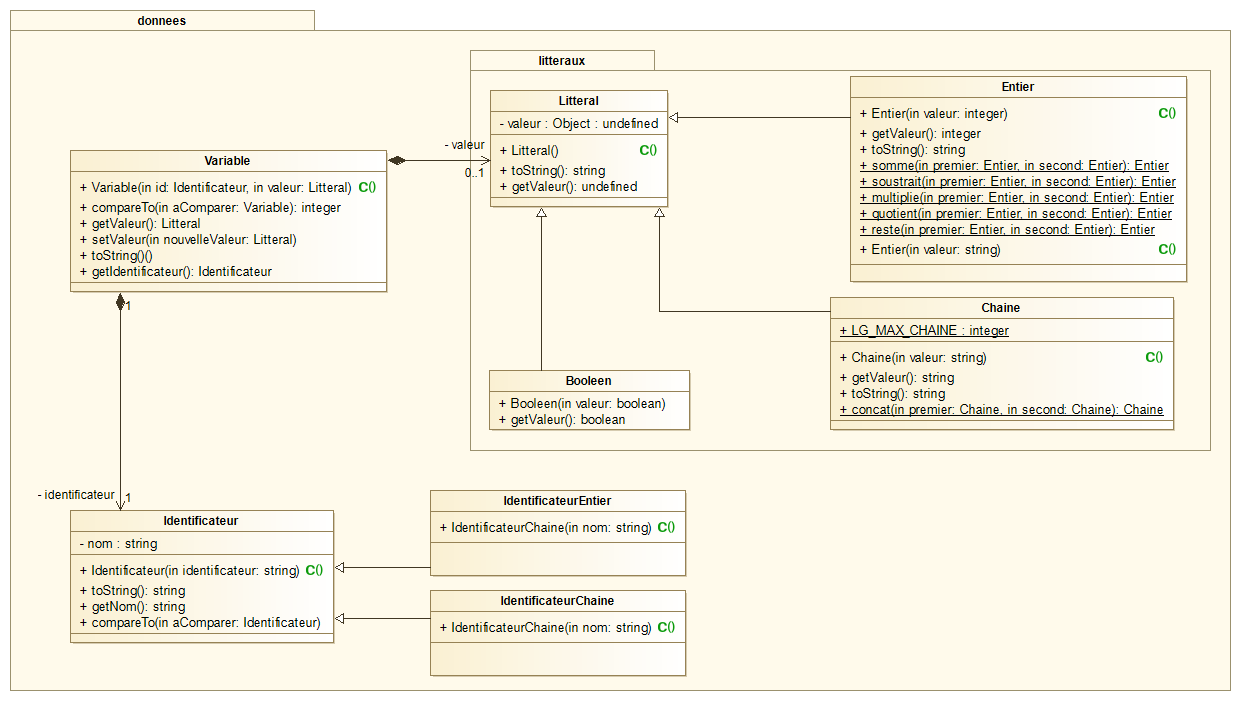
\includegraphics[scale=0.40]{./img/COO/COO_prototype_3/PackageDonnees}\end{center}
\par Le type booléen hérite de Litteral pour garder la logique de Litteral pouvant référencer chaque type de valeur du programme.

\section{Paquetage interpreteurlir.expressions} 
\begin{center}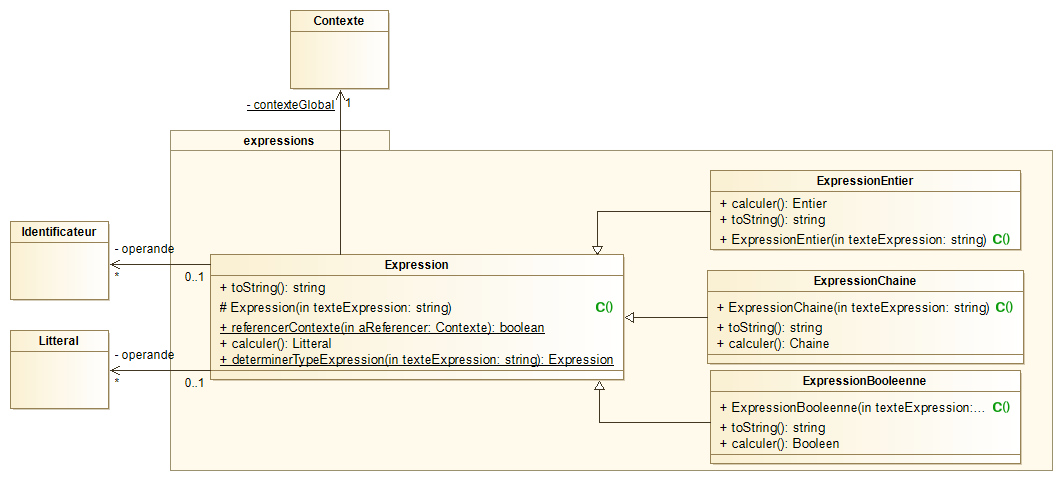
\includegraphics[scale=0.45]{./img/COO/COO_prototype_3/PackageExpression}\end{center}
\par L'expression booléenne ne s'obtient pas avec la méthode determinerExpression car celle-ci est utilisée que par si vaen qui utilise que ce type d'expression. Le constructeur d'ExpressionBooleenne est donc utilisé directement.

\section{Diagramme de classes général}
\begin{center}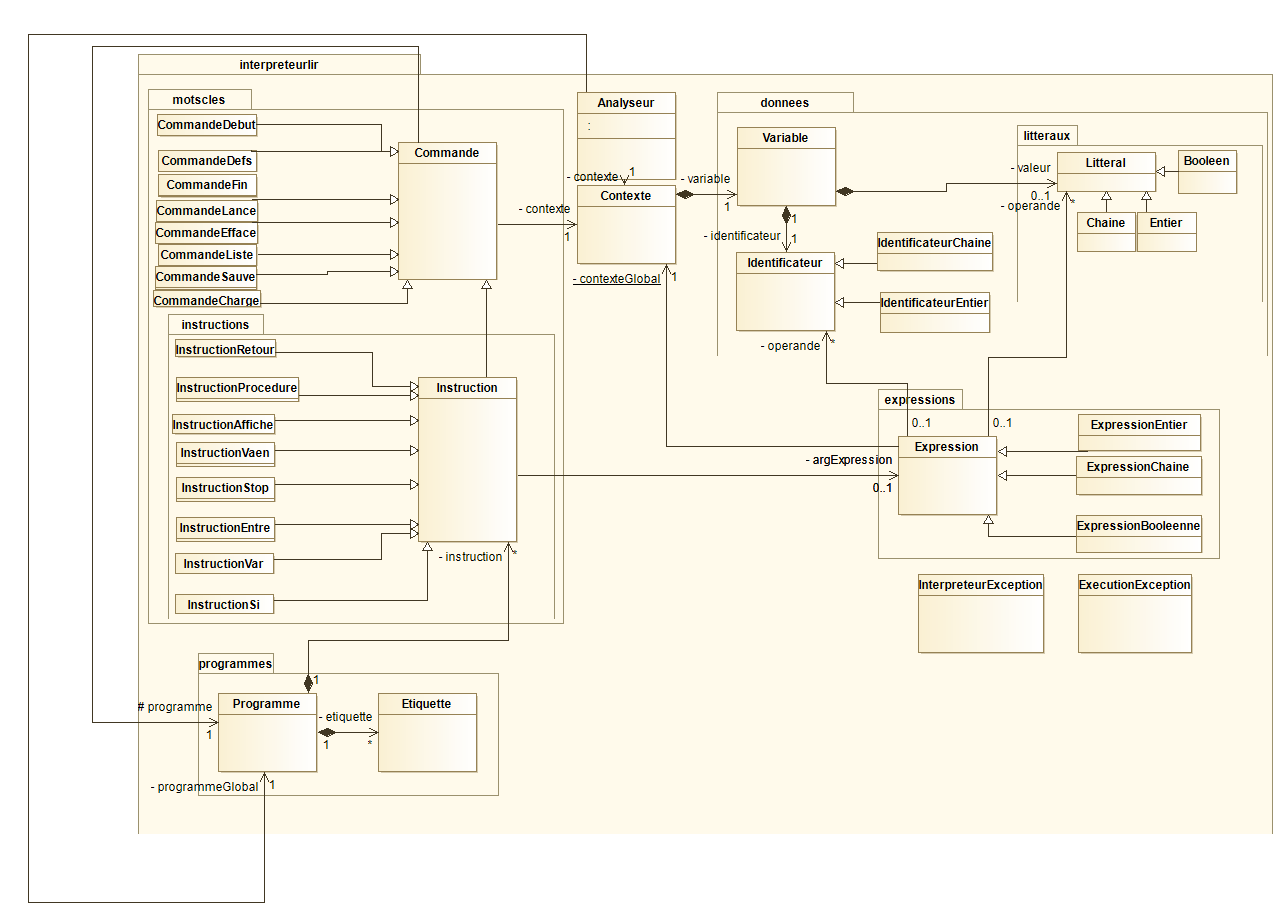
\includegraphics[scale=0.35]{./img/COO/COO_prototype_3/Scéma général simplifié}\end{center}
\par Les commandes sauve et charge ont été ajoutés à la conception mais sont similaires aux autres commandes. Pareil pour l'instruction si vaen. Ce diagramme général permet de voir l'ensemble de la conception pour ce qui est des associations et généralisation des classes.